\section{Grundlagen und Methoden} % (fold)
\label{sec:grundlagen_und_methoden}

	In den folgenden Kapiteln wird eine grundlegende Einführung und Definition der Verfahren gegeben, die für den weiteren Verlauf dieser Arbeit von Belang sind.
	Viele dieser Themen können hier nur angerissen werden, da ihre komplette Behandlung den Rahmen und das Ziel des Themas sprengen würden.
	Für eine genauere Einführung in die einzelnen Themengebiete, wird dem Leser geraten, sich mit den genannten Quellen auseinander zu setzen.

	\subsection{Szenengeometrie} % (fold)
	\label{sub:szenengeometrie}

		Um in einem Computer ein zweidimensionales Bild einer dreidimensionalen Umwelt oder auch \enquote{Szene} (engl.: \textit{scene}) zu generieren, benötigen wir ein mathematisches Modell, welches diese hinreichend gut beschreibt.
		Wir wollen uns einen Beobachter vorstellen, der die Umwelt und die Objekte in ihr von einem bestimmten Punkt im Raum aus betrachtet.
		Für viele Algorithmen, die diese Aufgabe lösen, ist dabei vor allem das Verhalten von Licht auf den Oberflächen dieser Objekte wichtig \cite{pbrt3, kajiya-lte, veach-thesis}.
		Der Einfachheit halber wollen wir davon ausgehen, dass Licht nur in den oberen Schichten eines Körpers mit dessen Material wechselwirkt.
		Diese Annahme reduziert die Komplexität des mathematischen Modells, die dann noch aus der Charakterisierung der Oberflächen besteht.

		Die Oberflächen realer physikalischer Körper sind im Allgemeinen beliebig geformt und können nicht in geschlossener Form durch eine Gleichung beschrieben werden.
		Dennoch lassen sie sich im analytischen Sinne durch einfachere Hyperflächen (engl.: \textit{shape} \cite[S.~123~ff]{pbrt3}) im Raum approximieren \cite{diffgeo}.
		Für die Bildgenerierung wählt man für solch eine Fläche meist ein Dreieck.
		Es ist einfach zu beschreiben und flexibel genug, um die meisten Objekte beliebig genau zu approximieren \cite{course-triangle-mesh, surface-triangle-mesh}.
		Dabei wollen wir entartete Dreiecke, die nur aus einem Punkt oder einer Strecke bestehen, ausschließen, da sie für die betrachteten Render-Verfahren nicht darstellbar sind.
		\begin{definition}[Dreieck]
			Ein Dreieck $\triangle$ wird durch eine Sequenz $(A,B,C)$ von Eckpunkten in $\SR^3$, für die die Menge $\set{B-A, C-A}$ linear unabhängig ist, charakterisiert.
			Seien weiterhin
			\[
				M \define \set[u+v\leq 1]{(u,v)\in[0,1]^2}
			\]
			\[
				\func{\varphi}{M}{\SR^3},\qquad \varphi(u,v) \define (1-u-v)A + uB + vC
			\]
			Dann ist die Menge der Punkte $S$ des Dreiecks gegeben durch $\im\varphi$ und $(M,\varphi)$ stellt deren Standardparametrisierung dar.
			Der Notation wegen, identifizieren wir $\triangle$ mit $S$ und definieren für alle $(u,v)\in M$
			\[
				\triangle(u,v) \define \varphi(u,v)
			\]
			Die baryzentrischen Koordinaten $(u,v,w)$ eines Punktes $x\in \triangle$ sind weiterhin durch die folgenden Eigenschaften gegeben.
			\[
				(u,v)\in M,\qquad w = 1-u-v,\qquad \triangle(u,v) = x
			\]
			Die analytische äußere Normale oder auch Normale ist definiert durch
			\[
				\mu \define \frac{\crossp{(B-A)}{(C-A)}}{\norm{\crossp{(B-A)}{(C-A)}}}
			\]
		\end{definition}

		Jedes Dreieck besitzt auf seiner gesamten Fläche eine eindeutige konstante äußere analytische Normale.
		Für die Simulation von globalen Beleuchtungseffekten ist diese Eigenschaft jedoch ein Nachteil, weil die Beleuchtung eines Objektes stark vom Verlauf seiner Normalen abhängt.
		Nähern wir ein Objekt durch $n\in\SN$ Dreiecke an, so nähern wir auch den Normalenverlauf des Objektes durch die stückweise konstanten Normalen der Dreiecke an.
		Der Fehler dieser Approximation tritt in Form eines facettenartigen Musters auf, welches für das menschliche Auge gut erkennbar ist \cite[S.~166]{pbrt3}.
		In Abbildung \ref{fig:facette} wird dieser Effekt genauer an einem Beispiel demonstriert.
		Folglich muss darauf geachtet werden, dass bei stetig differenzierbaren Oberflächen die Stetigkeit der Normalen erhalten bleibt \cite[S.~39~ff]{diffgeo}.
		\begin{definition}[Normalen-Funktion / Shading-Normale]
			Sei $\triangle$ ein Dreieck mit der Normalen $\mu$.
			Dann wird $\func{\nu}{\triangle}{\shs{\mu}}$ als Normalen-Funktion oder auch als Shading-Normale von $\triangle$ bezeichnet.
		\end{definition}

		\begin{figure}
			\begin{subfigure}[b]{0.5\textwidth}
				\center
				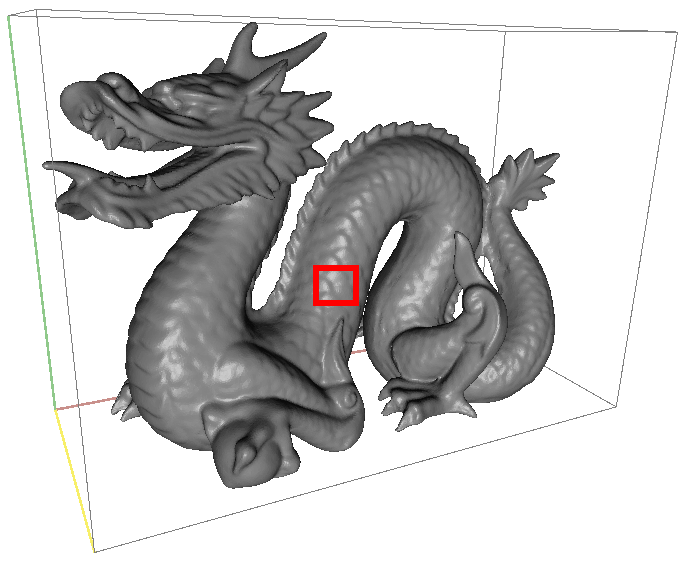
\includegraphics[width=0.95\textwidth]{pic/normal_facette-mark.png}
				% \caption{}
			\end{subfigure}
			\begin{subfigure}[b]{0.5\textwidth}
				\center
				
\includegraphics[width=0.95\textwidth]{pic/normal_facette-zoom.png}
				% \caption{}
			\end{subfigure}
			\caption[Facetten-Muster der \enquote{Dragon}-Szene ohne Shading-Normale]{Die Bilder zeigen die gerenderte \enquote{Dragon}-Szene. Das rechte Bild entspricht dem roten Bereich des Linken. In dieser Szene werden die Normalen des Objektmodells durch die analytischen Normalen der Dreiecke angenähert. Da das Modell sehr fein trianguliert ist, fällt dies im ersten Bild nicht auf. Zoomt man jedoch mit der Kamera heran, werden die Fehler durch die Approximation deutlich und die einzelnen Dreiecke sind mit dem menschlichen Auge auszumachen.}
			\label{fig:facette}
		\end{figure}

		Nach den Quellen \cite[S.~166,~584~ff]{pbrt3} und \cite[S.~38~ff,~183~ff]{real-time-render} sind die typischen Verfahren für eine genauere Interpolation die \enquote{Vertex-Shading-Normale} und das \enquote{Bump Mapping} (engl.: \textit{bumb mapping}).
		Formal gesehen, werden bei beiden Verfahren die Normalen der vorhandenen Geometrie durch eine Normalen-Funktion ersetzt.
		\begin{definition}[Vertex-Shading-Normale]
			Seien $\triangle$ ein Dreieck mit der Normalen $\mu$ und $\mu_A, \mu_B, \mu_C \in \shs{\mu}$ Normalen an den Eckpunkten des Dreiecks.
			Sei weiterhin $\nu$ eine Shading-Normale auf $\triangle$, sodass für alle $x\in \triangle$ mit den baryzentrischen Koordinaten $(u,v,w)$ gilt
			\[
				\nu(x) \define \frac{w\mu_A + u\mu_B + v\mu_C}{\norm{w\mu_A + u\mu_B + v\mu_C}}
			\]
			Dann ist $\nu$ stetig und man nennt es eine Vertex-Shading-Normale von $\triangle$.
		\end{definition}

		Durch das Setzen der Normalen an den Eckpunkten (engl.: \textit{vertex}) eines Dreiecks können wir sicher gehen, dass der Verlauf der Normalen stetig von einem Dreieck zu einem anderen übergeht.
		Ein beipielhafter Verlauf einer Vertex-Shading-Normalen wird in Abbildung \ref{fig:normal-function} gezeigt.
		Zu beachten ist, dass die Vektoren der Shading-Normale im Allgemeinen nicht mehr senkrecht auf der Geometrie stehen.
		Dadurch kann es, wie in \cite[S.~574~ff]{pbrt3} und \cite[S.~150~ff]{veach-thesis} gezeigt, zu Artefakten bei der Generierung des Bildes kommen.

		\begin{figure}
			\begin{subfigure}[b]{0.5\textwidth}
				\center
				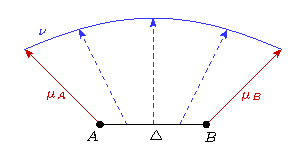
\includegraphics{gg_fig/scheme_normal-function_1.pdf}
				% \caption{Verlauf}
			\end{subfigure}
			\begin{subfigure}[b]{0.5\textwidth}
				\center
				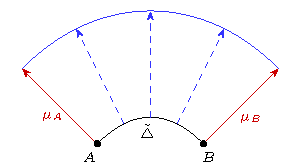
\includegraphics{gg_fig/scheme_normal-function_2.pdf}
				% \caption{approximierte Fläche}
			\end{subfigure}
			\caption[Beispiel des Verlaufs einer Vertex-Shading-Normalen]{Die erste Skizze auf der linken Seite zeigt den Verlauf einer Vertex-Shading-Normalen $\nu$ anhand eines Beispiels. $A$ und $B$ sind dabei zwei Eckpunkte eines Dreiecks $\triangle$. $\mu_A$ und $\mu_B$ sind die jeweilig gegebenen Vertex-Normalen an den Eckpunkten. Im rechten Bereich der Abbildung ist die durch $\nu$ approximierte gekrümmte Fläche $\tilde{\triangle}$, auf der die Shading-Normale $\nu$ senkrecht steht, eingezeichnet.}
			\label{fig:normal-function}
		\end{figure}

		Der letzte Schritt zur vollständigen Beschreibung der Szenengeometrie besteht darin, eine Menge von Dreiecken zu bilden, sodass diese ein physikalisches Objekt gut genug approximieren.
		In \cite{pbrt3} und \cite{course-triangle-mesh} werden solche Mengen auch \enquote{Mesh} (engl.: \textit{triangle mesh}) genannt.
		\begin{definition}[Mesh]
			Seien $n\in\SN$ und Dreiecke $\triangle_i$ mit Shading-Normalen $\nu_i$ für alle $i\in\SN,i\leq n$.
			Weiterhin definieren wir
			\[
				\e{T}\define \bigcup_{i=1}^n \triangle_i \qquad \e{A}\define \set[{ \exists!\ i\in\SN,i\leq n\colon\ x\in\triangle_i }]{x\in\e{T}}
			\]
			\[
				\func{\nu}{\e{T}}{\ssp\cup\set{0}},\qquad \nu(x)\define \sum_{i=1}^n \nu_i(x)\mathds{1}_{\e{A}\cap\triangle_i}(x)
			\]
			Dann nennen wir $\e{T}$ eine Mesh mit der Shading-Normalen $\nu$, wenn für $\sigma$-fast-alle $x\in\e{T}$ auch $x\in\e{A}$ gilt.
		\end{definition}

		Die Definition der Mesh verbietet, dass die Schnittpunkte der Dreiecke eine eigene Fläche im Raum bilden.
		So können wir sicher gehen, dass die Integration über die Punkte der Mesh eine eindeutige Lösung ergibt.
		Es ist jedoch erlaubt, dass sich Dreiecke in einem Punkt oder einer Strecke schneiden dürfen.
		Dies ist auch nötig, um komplexere Objekte formen zu können.
		In der Praxis ist die genannte Bedingung im Allgemeinen erfüllt und folglich auch keine fundamentale Einschränkung \cite{pbrt3,course-triangle-mesh,surface-triangle-mesh,veach-thesis}.

	% subsection szenengeometrie (end)

	\subsection{Streuung von Licht an Oberflächen} % (fold)
	\label{sub:bsdf}

		Im letzten Abschnitt wurden die Grundbausteine einer Szene eingeführt, die deren Geometrie beschreiben.
		Wie bereits erwähnt, benötigen wir jedoch zusätzlich die Informationen, auf welche Art und Weise Licht mit den Oberflächen der Objekte interagiert.
		Dieses Verhalten wird durch die sogenannte \enquote{Bidirektionale Streuungsverteilungsfunktion} (engl.: \textit{bidirectional scattering distribution function}, BSDF), die sich aus einer \enquote{Bidirektionalen Reflektanzverteilungsfunktion} (engl.: \textit{bidirectional reflectance distribution function}, BRDF) und einer \enquote{Bidirektionalen Transmissionsverteilungsfunktion} (engl.: \textit{bidirectional transmittance distribution function}, BTDF) zusammensetzt, geklärt.
		Strukturierte Einführungen zu diesem Thema erhält man in den Quellen \cite{pbrt3,veach-thesis,real-time-render,intro-brdf,radiosity}.
		\begin{definition}
			Sei $\mu\in\ssp$ die Normale am Punkt einer Oberfläche.
			Dann ist eine BSDF bezüglich $\mu$ gegeben durch eine integrierbare Abbildung $\func{f}{\ssp\times\ssp}{[0,\infty)}$ mit den folgenden Eigenschaften.

			\begin{enumerate}[label = \normalfont{(\roman*)}]
				\item
				Für $\sigma^2$-fast-alle $(\omega_\m{i},\omega_\m{o})$ mit $\omega_\m{i}\in\ssp$, $\omega_\m{o}\in\shs{\nu}$ und $\nu\define\sign(\dotp{\mu}{\omega_\m{i}})\cdot\mu$ gilt
				\[
					f(\omega_\m{i},\omega_\m{o}) = f(\omega_\m{o},\omega_\m{i}) \hfill \text{(Helmholtz-Reziprozität)}
				\]

				\item
				Für $\sigma$-fast-alle $\omega_\m{i}\in\ssp$ gilt
				\[
					\integral{\ssp}{}{f(\omega_\m{i},\omega) \abs{\dotp{\mu}{\omega}}}{\sigma(\omega)} \leq 1 \hfill \text{(Energieerhaltung)}
				\]
			\end{enumerate}
		\end{definition}

		Eine BSDF $f$ gibt an, welcher Anteil des einfallenden Lichtes aus der Richtung $\omega_\m{i}\in\ssp$ in die Richtung $\omega_\m{o}\in\ssp$ gestreut wird.
		Gilt dabei $\omega_\m{o}\in\shs{\nu}$, so befindet sich $\omega_\m{o}$ in der gleichen Hemisphäre bezüglich $\mu$ wie $\omega_\m{i}$ und es handelt sich um eine Reflexion des Lichtes.
		Der verbleibende Fall beschreibt die Transmission.
		Die BSDF stellt damit eine Verallgemeinerung der idealen Reflexion und Brechung an Oberflächen dar.
		Die Quellen \cite[S.~571~ff]{pbrt3} und \cite[S.~135~ff]{veach-thesis} weisen zudem nach, dass die Helmholtz-Reziprozität nur für den reflektierten Anteil des Lichtes gilt.
		In Abbildung \ref{fig:brdf} ist das Beispiel einer typischen BSDF gezeigt, die keine Transmission des Lichtes zulässt \cite[S.~509~ff]{pbrt3}.

		\begin{figure}
			\center
			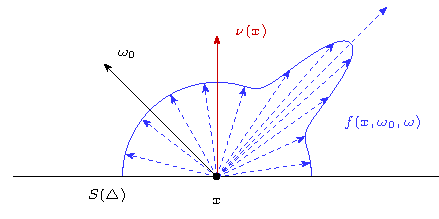
\includegraphics{gg_fig/brdf_1.pdf}
			\caption[Schema einer BSDF]{Die Abbildung zeigt die Verteilung des reflektierten Lichtes für alle $\omega\in\shs{\mu}$ bezüglich einer konstanten Einfallsrichtung $\omega_\m{i}\in\shs{\mu}$ einer BSDF $f$ bezüglich der Oberflächennormalen $\mu\in\ssp$.}
			\label{fig:brdf}
		\end{figure}

		Die hier eingeführten Funktionen für die Charakterisierung von Materialien können auf verschiedene Weisen verallgemeinert werden.
		Zu beachten ist vor allem die fehlende Abhängigkeit von der Wellenlänge des einfallenden und der des gestreuten Lichtes, durch welche Effekte wie Dispersion, Irisieren und Lumineszenz verhindert werden.
		Ein weiteres physikalisches Phänomen stellt die Volumenstreuung dar.
		Bei der Betrachtung dieser wird ein Material durch die sogenannte \enquote{BSSRDF} beschrieben \cite[S.~671~ff]{pbrt3}.

		BSDFs sind im Allgemeinen nicht in geschlossener Form formulierbar \cite[S.~507~f]{pbrt3}.
		Aus diesem Grund wollen wir für die Konstruktion realistischer Materialien, wie bei der Approximation von Oberflächen, verschiedene einfache BSDFs zu Grunde legen.
		In den beiden folgenden Beispielen handelt es sich um die BSDFs $f$ bezüglich der Normalen $\mu\in\ssp$ für die Lambertsch diffuse Reflexion (engl.: \textit{Lambertian reflection}, \cite[S.~531~f]{pbrt3}) und für die ideale Reflexion (engl.: \textit{specular reflection}, \cite[S.~144~f]{veach-thesis}).
		Weitere BSDF-Modelle sind in \cite{pbrt3,veach-thesis,radiosity} zu finden.
		Es seien $\omega_\m{i},\omega_\m{o}\in\ssp$ mit $\nu\define\sign(\dotp{\mu}{\omega_\m{i}})\cdot\mu$ gegeben.
		\[
			f(\omega_\m{i},\omega_\m{o}) = \frac{1}{\pi}\mathds{1}_{\shs{\nu}}(\omega_\m{o}) \hfill \text{(Lambertsch diffuse Reflexion)}
		\]
		\[
			f(\omega_\m{i},\omega_\m{o}) = \frac{\delta_{\omega_\m{o}}(2\dotp{\mu}{\omega_\m{i}}\mu - \omega_\m{i})}{\abs{\dotp{\mu}{\omega_\m{i}}}} \hfill \text{(ideale Reflexion)}
		\]

	% subsection bsdf (end)

	\subsection{Beleuchtung und Szene} % (fold)
	\label{sub:beleuchtung_und_szene}

		Die BSDF an einem Punkt beschreibt lediglich die Streuung des einfallenden Lichtes.
		Um den Render-Verfahren einen Sinn zu geben, benötigen wir demnach Lichtquellen.
		In den Quellen \cite[S.~707~ff]{pbrt3} und \cite{course-photon-map} werden verschiedene Arten von Lichtquellen definiert, implementiert und gesamplet.
		Der einfachste Weg Lichtquellen einzuführen, besteht in einer abstrakten Formulierung, die unabhängig von der Szenengeometrie agiert.
		Wir wollen eine sogenannte \enquote{Umgebungsbeleuchtung} (engl.: \textit{HDR environment map} oder \textit{infinite area light}, \cite[S.~737~f]{pbrt3}) einführen.
		\begin{definition}[Umgebungsbeleuchtung]
			Sei $\func{f}{(0,\infty)\times\ssp}{[0,\infty)}$ eine integrierbare Abbildung. Dann wird $f$ eine Umgebungsbeleuchtung genannt.
			% Eine Umgebungsbeleuchtung ist definiert als eine integrierbare Abbildung $\func{f}{(0,\infty)\times\ssp}{[0,\infty)}$.
		\end{definition}

		Diese Funktion beschreibt das Licht verschiedener Wellenlängen, welches von einer Kugeloberfläche mit quasi unendlich großem Radius in die Szene ausgesandt wird.
		Für einen Punkt der Szene ist dessen Beleuchtung durch diese Funktion also unabhängig von dessen Position.
		Diese Tatsache wird in Abbildung \ref{fig:hdr_environment_map} wieder an einem Beispiel gezeigt.

		\begin{figure}
			\center
			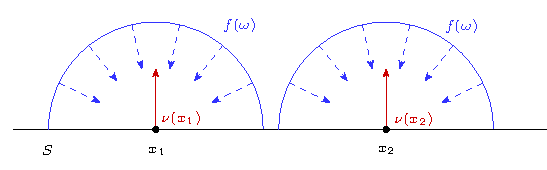
\includegraphics{gg_fig/hdr_environment_map_1.pdf}
			\caption[Wirkungsweise einer Umgebungsbeleuchtung]{Die Darstellung zeigt, dass die Beleuchtung zweier Punkte $x_1$ und $x_2$ einer Oberfläche $S$ mit den Normalen $\nu(x_1)$ und $\nu(x_2)$ durch eine Umgebungsbeleuchtung $f$ nur abhängig von der Verdeckung der Punkte und nicht von deren Position ist. Bei $x_1$ und $x_2$ sind in diesem Falle die gleichen Lichtintensitäten zu messen. Es ist $\lambda\in(0,\infty)$ die Wellenlänge des Lichtes und $\omega\in\ssp$ der Raumwinkel.}
			\label{fig:hdr_environment_map}
		\end{figure}

		Aber auch die Materialien der Szene sollten in der Lage sein Licht auszusenden.
		Wir führen dementsprechend eine Abbildung ein, die die benötigten Eigenschaften erfüllt.
		Häufig werden diese Lichtquellen auch \enquote{Feldlichtquellen} (engl.: \textit{area light}) genannt \cite[S.~733~ff]{pbrt3}.
		\begin{definition}[Emission]
			Sei $\e{T}$ eine Mesh mit einer Shading-Normalen $\nu$.
			Dann ist eine Emission von $\e{T}$ durch eine integrierbare Abbildung $\func{E}{\e{T}\times(0,\infty)\times\ssp}{[0,\infty)}$ gegeben.
		\end{definition}

		Wie bei der vorherigen Definition beschreibt diese Funktion das ausgesandte Licht in Abhängigkeit der Wellenlänge und des Raumwinkels.
		Der Unterschied besteht darin, dass sie auf der Oberfläche einer Mesh variieren kann und sich damit auch die Beleuchtung eines Punktes je nach Position verändert.

		Durch die Einführung der Lichtquellen erhalten wir nun die vollständige Beschreibung einer Szene durch Zusammenführung der bereits definierten Strukturen.
		\begin{definition}[Szene]
			Eine Szene ist ein Tupel $(\e{T},\nu,f,E,U)$, bestehend aus einer Mesh $\e{T}$ mit einer Shading-Normalen $\nu$, einer integrierbaren Abbildung $\func{f}{\e{T}\times\ssp\times\ssp}{[0,\infty)}$, wobei $f(x,\cdot,\cdot)$ für $\sigma$-fast-alle $x\in\e{T}$ ein BSDF bezüglich $\nu(x)$ darstellt, einer Emission $E$ von $\e{T}$ und einer Umgebungsbeleuchtung $U$.
		\end{definition}

	% subsection beleuchtung_und_szene (end)

	\subsection{Raytracing} % (fold)
	\label{sub:raytracing}

		Im einfachsten Falle bezeichnet das Wort \enquote{Raytracing} (engl.: \textit{ray tracing}) einen Algorithmus zur Ermittlung der Sichtbarkeit von dreidimensionalen Objekten bezüglich eines Ursprungspunktes (engl.: \textit{origin}) im Raum \cite{pbrt3,parker-ray-tracing}.
		Häufig versteht man darunter jedoch auch eine Render-Technik für die Generierung eines gesamten Bildes aus einer gegebenen Szene, die auf dem eben genannten Raytracing-Algorithmus basiert \cite{pbrt3, nikodym-ray-tracing, parker-ray-tracing}.

		Grundsätzlich gibt es viele Verfahren, um ein Szene auf ein Bild zu rendern \cite{survey-visibility,real-time-render}.
		Die Erfahrung zeigt aber, dass vor allem in Bereichen, in denen die globalen Beleuchtungseffekte realistisch simuliert werden sollen, Raytracing eine wichtige Grundlage darstellt.
		Der Grund dafür besteht in der Tatsache, dass Raytracing das \enquote{Sichtbarkeitsproblem} (engl.: \textit{visibility problem}, \cite{3d-visibility, survey-visibility}) löst und durch die Verwendung von Strahlen eine Basis für die Lichtberechnung im Sinne der geometrischen Optik bereitstellt \cite{pbrt3,veach-thesis,parker-ray-tracing}.
		\begin{definition}[Sichtbarkeitsproblem]
			Sei $\e{T}$ eine Mesh.
			Dann ist die Sichtbarkeitsfunktion von $\e{T}$ die folgende Abbildung.
			\[
				\func{V_\e{T}}{\SR^3\times\e{T}}{\set{0,1}}
			\]
			\[
				V_\e{T}(o,x)=
				\begin{cases}
					1 &: \e{T} \cap \set[\gamma\in(0,1)]{(1-\gamma)o + \gamma x} = \emptyset \\
					0 &: \m{sonst}
				\end{cases}
			\]
			Das Sichtbarkeitsproblem beschreibt die Aufgabe diese Funktion für gegebene Parameter zu evaluieren.
		\end{definition}

		Die Sichtbarkeitsfunktion gibt an, ob der Oberflächenpunkt $x$ vom Beobachtungspunkt $o$ aus in gerader Linie gesehen werden kann oder ob zwischen diesen Punkten ein weiterer Punkt der Mesh $\e{T}$ den Punkt $x$ verdeckt \cite[S.~30]{3d-visibility}.
		Daran anknüpfend besteht die Basis des Raytracing-Verfahrens auf dem Aussenden von \enquote{Strahlen} (engl.: \textit{ray}) bezüglich eines Ursprungspunktes \cite{pbrt3,parker-ray-tracing,nikodym-ray-tracing}.
		Für diese Strahlen kann der Schnittpunkt mit $\e{T}$ ermittelt werden.
		Liegt der Schnittpunkt zwischen $o$ und $x$, so beträgt der Wert der Sichtbarkeitsfunktion $0$.
		Im noch bleibenden Fall ergibt sich der Wert zu $1$.
		Die Sichtbarkeitsfunktion kann somit für alle gegebenen Parameter durch Raytracing berechnet werden.
		Abbildung \ref{fig:ray_tracing-1} zeigt diese Methode anhand einer Skizze.

		\begin{figure}
			\center
			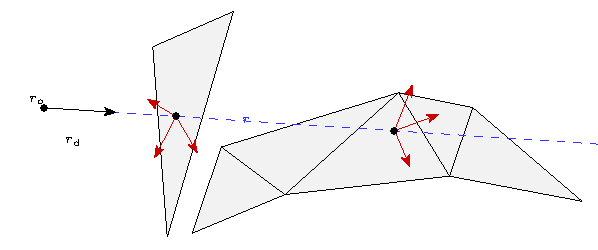
\includegraphics{gg_fig/ray_tracing_1.pdf}
			\caption[Skizze des Sichtbarkeitsproblems und des Raytracing-Verfahrens]{Die Abbildung zeigt eine Skizze, welche das Sichtbarkeitsproblem und den Raytracing-Algorithmus verdeutlicht. Die grau melierten Dreiecke sollen die gegebene Mesh $\e{T}$ darstellen. Der ausgesendete Strahl $r$, gegeben durch $(r_\m{o},r_\m{d})$, trifft in der Mesh genau zwei Punkte $x_1$ und $x_2$. Dabei wird $x_2$ durch $x_1$ verdeckt. Es gilt also $V_\e{T}(r_\m{o},x_1)=1$ und $V_\e{T}(r_\m{o},x_2)=0$.}
			\label{fig:ray_tracing-1}
		\end{figure}

		\begin{figure}
			\center
			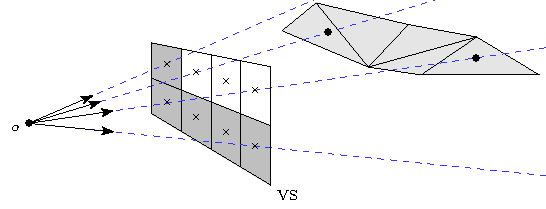
\includegraphics{gg_fig/ray_tracing_2.pdf}
			\caption[Raytracing als Render-Verfahren]{In der Skizze ist ein typisches Render-Verfahren auf der Basis des Raytracing-Algorithmus dargestellt. Bezüglich eines Beobachtungspunktes $o\in\SR^3$ wird durch jeden Pixel eines virtuellen Bildschirms $\m{VS}$ ein Strahl geschossen und der Wert der Raytracing-Funktion evaluiert. Die grau melierten Dreiecke bilden die Mesh $\e{T}$. Je nachdem, ob ein Strahl einen Schnittpunkt mit $\e{T}$ aufweist, wird ein entsprechendes Shading-Verfahren ausgeführt. Der Übersicht wegen sind im Bild nur vier der eigentlich acht Strahlen sichtbar.}
			\label{fig:ray_tracing-2}
		\end{figure}

		\begin{definition}[Strahl]
			Seien ein Ursprung $o\in\SR^3$, eine Richtung $d\in\ssp$ und die folgende Abbildung gegeben.
			\[
				\func{\varphi}{[0,\infty)}{\SR^3},\qquad \varphi(\gamma)\define o + \gamma d
			\]
			Dann wird das Bild $\im\varphi$ ein Strahl $r$ genannt.
			Dabei ist $([0,\infty),\varphi)$ die Standardparametrisierung von $r$.
			Der Notation wegen, definieren wir für alle $\gamma\in[0,\infty)$
			\[
				r(\gamma) \define \varphi(\gamma)
			\]
			Durch das Tupel $(o,d)$ charakterisieren und identifizieren wir den Strahl $r$.
			Die Menge aller Strahlen definieren wir durch $\e{R}$.
		\end{definition}

		Die vollständige Evaluierung von $V_\e{T}$ ist jedoch häufig nicht notwendig.
		In Abbildung \ref{fig:ray_tracing-1} ist klar, dass alle Punkte von $r$, die hinter $x_1$ liegen, vom Beobachtungspunkt $r_\m{o}$ aus nicht sichtbar sind.
		Beim eigentlichen Raytracing-Algorithmus wirkt sich diese Eigenschaft positiv aus.
		Es reicht, für eine gegebene Richtung und einen gegebenen Beobachtungspunkt den nächsten Schnittpunkt des resultierenden Strahles zu ermitteln.
		Für alle weiteren Schnittpunkte ergibt sich, sofern diese existieren, die Sichtbarkeitsfunktion zu Null, wodurch diese Punkte im weiteren Vorgehen ignoriert werden können \cite[S.~4~ff,~866]{pbrt3}.
		\begin{definition}[Raytracing-Funktion]
			Sei $\e{T}$ eine Mesh.
			Dann ist die Raytracing-Funktion von $\e{T}$ durch die folgende Abbildung gegeben.
			\[
				\func{\m{rt}_\e{T}}{\e{R}}{(0,\infty]}
			\]
			\[
				\m{rt}_\e{T}(r) \define
				\begin{cases}
					\min\set[r(\gamma)\in \e{T}]{\gamma\in(0,\infty)} &: \e{T}\cap (r\setminus\set{r(0)}) \neq \emptyset \\
					\infty &: \m{sonst}
				\end{cases}
			\]
		\end{definition}

		Wie bereits erwähnt, erweitert man diesen Algorithmus häufig mit der Berechnung eines gesamten Bildes, indem man für jeden Pixel des Bildes einen oder mehrere Strahlen durch einen analogen virtuellen Pixel im Szenenraum schießt und die Raytracing-Funktion für diese evaluiert \cite{pbrt3,parker-ray-tracing,nikodym-ray-tracing}.
		Abbildung \ref{fig:ray_tracing-2} zeigt dieses Verfahren anhand einer Skizze.
		Um gleichzeitig das sogenannte \enquote{Shading} zu ermöglichen, ermittelt man nicht nur den Schnittpunkt, sondern auch in welchem Dreieck sich dieser befindet und welche baryzentrischen Koordinaten er besitzt \cite{pbrt3,ray-triangle-intersection}.
		Die Implementierung des Raytracing-Verfahrens soll hier nicht gezeigt werden, da eine einfache Implementierung einen zu großen Rechenaufwand darstellt und die hier verwendete optimierte Variante weit über das Thema dieser Arbeit hinausgeht.
		Für eine strukturierte Einführung von Beschleunigungsstrukturen sei auf \cite[S.~247~ff]{pbrt3} und \cite{parker-ray-tracing,nikodym-ray-tracing} verwiesen.

	% subsection raytracing (end)

	\subsection{Radiometrie} % (fold)
	\label{sub:radiometrie}

		Ein physikalischer Körper $K$ mit der Oberfläche $\partial K$ und äußerer Normalen-Funktion $\mu$ sendet aufgrund verschiedener physikalischer Effekte, wie zum Beispiel Reflexion oder Emission, elektromagnetische Wellen aus \cite{nolting-edyn}.
		Für die Simulation von Beleuchtungseffekten ist es nötig, die Abhängigkeit dieser Abstrahlung für verschiedene Wellenlängen $\lambda\in(0,\infty)$, verschiedene Oberflächenpunkte $x\in\partial K$ und verschiedene Richtungen $\omega\in\ssp$ zu betrachten.
		Dafür führen wir die sogenannte \enquote{spektrale Strahldichte} (engl.: \textit{spectral radiance}) ein.
		Sie gibt an, wie viel Energie pro Zeit, pro Wellenlängenänderung, pro Flächenelement und pro Raumwinkel abgestrahlt beziehungsweise empfangen wird \cite{intro-radiometry,malacara-colorimetry,ohta-colorimetry}.
		Sind also messbare Teilmengen $\Lambda\subset (0,\infty)$, $U\subset \partial K$ und $S\subset\ssp$ gegeben, so kann man die spektrale Strahldichte über die abgegebene Strahlungsleistung $\Phi(U,\Lambda,S)$ der Oberfläche $U$ in den Raumwinkelbereich $S$ definieren \cite{intro-radiometry}.
		Die zugehörige Abbildung ist dann wie folgt gegeben.
		\[
			\func{\s{L}}{\partial K\times(0,\infty)\times \ssp}{[0,\infty)}
		\]
		\[
			\Phi(U,\Lambda,S) \definedby \integral{U}{}{ \integral{\Lambda}{}{ \integral{S}{}{ \s{L}(x,\lambda,\omega)\abs{\dotp{\mu(x)}{\omega}} }{\sigma(\omega)} }{\lambda(\lambda)} }{\sigma(x)}
		\]
		Abbildung \ref{fig:radiance} zeigt eine Skizze, welche die Struktur dieser Funktion verdeutlicht.
		Der Erfahrung nach stellt die spektrale Strahldichte für das menschliche Auge die sinnvollste messbare Größe für die empfundene Helligkeit einer Oberfläche bezüglich eines Beobachtungspunktes dar \cite{malacara-colorimetry,ohta-colorimetry}.

		\begin{figure}
			\center
			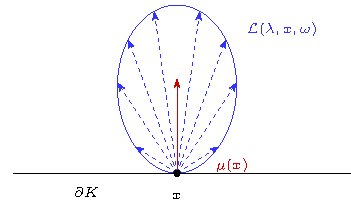
\includegraphics{gg_fig/radiance_1.pdf}
			\caption[Skizzenhaftes Beispiel der Strahldichte]{Die Skizze stellt das qualitative Beispiel einer spektralen Strahldichte $\s{L}$ dar, die an einem Punkt $x$ auf der Oberfläche $\partial K$ mit der äußeren Normalen $\mu(x)$ und für eine Wellenlänge $\lambda$ eine Verteilung in Abhängigkeit von $\omega\in\ssp$ besitzt.}
			\label{fig:radiance}
		\end{figure}

		Eine weitere Größe, die ich hier einführen möchte, ist die sogenannte spektrale \enquote{Bestrahlungsstärke} oder auch spektrale Irradianz (engl.: \textit{spectral irradiance}).
		Sie wird vor allem bei der noch folgenden Konstruktion der Irradiance Maps gebraucht werden.
		Wir definieren sie für eine messbare Teilmenge $S\subset\ssp$ \cite[S.~9~f]{guide-radiometry}.
		\[
			\func{\s{E}}{\partial K\times (0,\infty)}{[0,\infty)},\qquad \s{E}(x,\lambda) \define \integral{S}{}{ \s{L}(x,\lambda,\omega)\abs{\dotp{\mu(x)}{\omega}} }{\sigma(\omega)}
		\]
		Die spektrale Bestrahlungsstärke quantifiziert die Energie pro Zeit, pro Wellenlängenänderung und pro Flächenelement, die an einem Punkt auf der Oberfläche des Objektes aus dem Raumwinkelbereich $S$ empfangen wird \cite{intro-radiometry,guide-radiometry}.

		Für die weiteren Algorithmen und Implementierungen reicht es, entkoppelte Abbildungen zu betrachten, welche für jeden Punkt einer Szene und jede gegebene Richtung der Strahldichte beziehungsweise der Irradianz entsprechen.
		Später werden dies die Funktionen sein, die wir durch \enquote{Path Tracing} simulieren und durch eine Irradiance Map auf der Oberfläche speichern wollen.
		\begin{definition}[Strahldichte und Irradianz]
			Sei $\Sigma\define (\e{T},\nu,f,E,U)$ eine Szene.
			Dann ist eine Strahldichte von $\Sigma$ gegeben durch eine integrierbare Abbildung
			\[
				\func{L}{\e{T}\times(0,\infty)\times\ssp}{[0,\infty)}
			\]
			Die einfallende Strahldichte $\tilde{L}$ der Szene $\Sigma$ bezüglich $L$ wird für alle $x\in\e{T}$, $\lambda\in(0,\infty)$ und $\omega\in\ssp$ wie folgt formuliert.
			\[
				\tilde{L}(x,\lambda,\omega)\define
				\begin{cases}
					L(r(\m{rt}_\e{T}(r)),\lambda,-\omega) &: r\in\e{R}, r\equiv(x,\omega),\ \m{rt}_\e{T}(r) < \infty \\
					U(\lambda,\omega) &: \m{sonst}
				\end{cases}
			\]
			Die zu $L$ gehörige Irradianz definieren wir durch die folgende Funktion.
			\[
				\func{R}{\e{T}\times(0,\infty)}{[0,\infty)},\qquad R(x,\lambda)\define \integral{\shs{\nu(x)}}{}{\tilde{L}(x,\lambda,\omega)\dotp{\mu(x)}{\omega}}{\sigma(\omega)}
			\]
		\end{definition}

		In der Definition entspricht $\tilde{L}(x,\lambda,\omega)$ der aus $\omega$ einfallenden Strahldichte am Punkt $x$ der Wellenlänge $\lambda$.
		Die Funktionen $\tilde{L}$ und $L$ sind über die Raytracing-Funktion miteinander verbunden.
		Existiert jedoch für den gegebenen Strahl $r$ kein Schnittpunkt mit der Szene, so entspricht die einfallende Strahldichte gerade der Umgebungsbeleuchtung.
		In Abbildung \ref{fig:lte-incident-emitted-radiance} wird dieser Zusammenhang an einem Beispiel demonstriert.

		\begin{figure}
			\center
			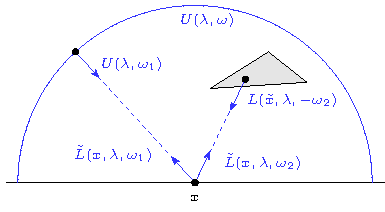
\includegraphics{gg_fig/lte-incident_and_emitted_radiance.pdf}
			\caption[Relation zwischen der ein- und ausfallenden Strahldichte]{Die Abbildung skizziert an einem Beispiel die Relation der Funktionen $L$ und $\tilde{L}$ aus der Definition der Strahldichte. Dabei stellen das Dreieck einen Teil der Mesh, $U$ die Umgebungsbeleuchtung für $\omega\in\ssp$, $\omega_1,\omega_2$ Raumrichtungen, $\lambda$ die betrachtete Wellenlänge und $x$ einen Punkt auf der Mesh dar. Für $\tilde{x}$ gilt nach Defintion $\tilde{x}=r(\m{rt}_\e{T}(r))$, wobei der Strahl $r$ durch $(x,\omega_2)$ gegeben ist. Der Strahl in Richtung $\omega_1$ besitzt keinen Schnittpunkt mit der Szene, wodurch sich die einfallende Strahldichte aus der Umgebungsbeleuchtung ergibt.}
			\label{fig:lte-incident-emitted-radiance}
		\end{figure}

	% subsection radiometrie (end)

	\subsection{Rendergleichung} % (fold)
	\label{sub:rendergleichung}

		Die \enquote{Rendergleichung} (engl.: \textit{rendering equation} oder \textit{light transport equation}, \cite[S.~861]{pbrt3}) ist eine Integralgleichung, die 1986 von James T. Kajiya entwickelt wurde, um die bis zu diesem Zeitpunkt verbreiteten Rendertechniken für die Simulation globaler Beleuchtungseffekte auf eine gemeinsame Basis zu stellen \cite{kajiya-lte}.
		In den Quellen \cite{kajiya-lte}, \cite[S.~349~ff,~862~ff]{pbrt3} und \cite{veach-thesis} wird sie mithilfe der Prinzipien der geometrischen Optik und dem Energieerhaltungssatz hergeleitet.
		Quelle \cite{veach-thesis} stellt dabei die resultierende Gleichung zusätzlich in einer Operator-Formulierung dar.
		Insbesondere handelt es sich bei der Rendergleichung um eine Fredholm-Integralgleichung 2.Art, die damit unter gewissen Voraussetzungen eine eindeutige Lösung besitzt (siehe hierzu \cite[S.~103~ff]{veach-thesis} und \cite{integral-equations}).

		\begin{definition}[Rendergleichung]
			Seien $\Sigma\define (\e{T},\nu,f,E,U)$ eine Szene und $L$ eine Strahldichte von $\Sigma$.
			Dann gehorcht $L$ der Rendergleichung, wenn für alle $x\in\e{T}$, $\lambda\in(0,\infty)$ und $\omega_\m{o}\in\ssp$ das Folgende gilt.
			\[
				L(x,\lambda,\omega_\m{o}) = E(x,\lambda,\omega_\m{o}) + \integral{\ssp}{}{ f(x,\omega,\omega_\m{o})\tilde{L}(x,\lambda,\omega) \abs{\dotp{\nu(x)}{\omega}} }{\sigma(\omega)}
			\]
		\end{definition}

		Die Strahldichte in Richtung $\omega$ entspricht damit der Summe des emittierten und des gestreuten Lichtes am Punkt $x$.
		Gehorcht die Strahldichte einer Szene der Rendergleichung, so simuliert sie die globalen Beleuchtungseffekte dieser Szene auf einer physikalischen Basis, wodurch die entstehenden Lichtverhältnisse für das menschliche Auge real wirken \cite{kajiya-lte,pbrt3,veach-thesis}.
		Die Rendergleichung lässt sich aber im Allgemeinen nicht analytisch lösen \cite{pbrt3,veach-thesis,kajiya-lte}.
		% In \cite[S.~863~f]{pbrt3} ist jedoch die Lösung eines Spezialfalls beschrieben.
		Aus diesem Grund sind verschiedene numerische Lösungsmethoden für die Berechnung einer Strahldichte, die der Rendergleichung gehorcht, entwickelt worden.
		Die berühmtesten Beispiele stellen das \enquote{Path Tracing} \cite{kajiya-lte}, das \enquote{Bidirectional Path Tracing} \cite{bidirectional-path-tracing}, der \enquote{Metropolis Light Transport} \cite{veach-mlt} und das \enquote{Photon Mapping} \cite{course-photon-map} dar.
		Eine strukturierte Einführung zu diesen Verfahren gibt es auch hier in \cite{pbrt3}.
		Das Beispiel für eine durch Path Tracing erzeugte Lösung ist in Abbildung \ref{fig:example-audi-r8-pt} zu sehen.

		\begin{figure}
			\center
			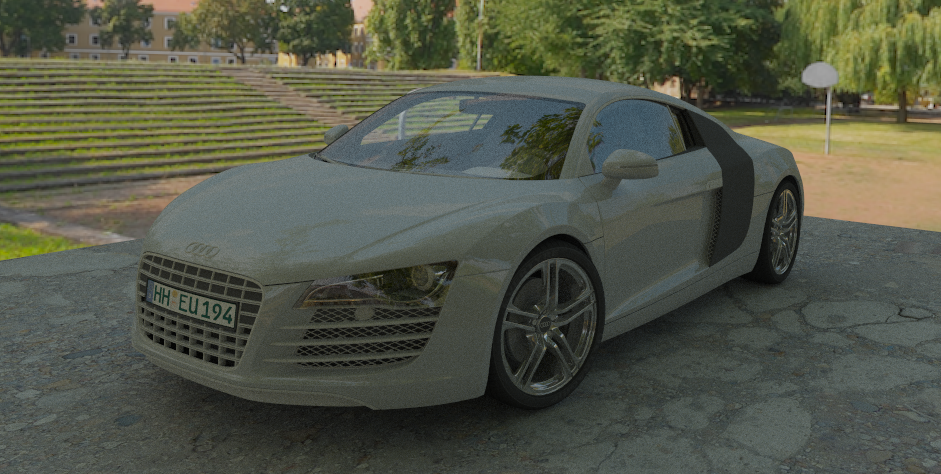
\includegraphics[width=0.95\textwidth]{pic/example-audi_r8-pt.png}
			\caption[Path Tracing am Beispiel der \enquote{Audi R8}-Szene mit \enquote{Basketball Court}-HDR]{Die Abbildung stellt eine durch Path Tracing simulierte Lösung der Rendergleichung für die \enquote{Audi R8}-Szene mit \enquote{Basketball Court}-HDR dar. Für die BSDFs ist immer eine Mischung aus idealer Reflexion, Lambertsch diffuser Reflexion und idealer Brechung gewählt worden.}
			\label{fig:example-audi-r8-pt}
		\end{figure}

		Alle genannten Verfahren arbeiten auf der Basis von Zufallszahlen.
		Da die Rendergleichung eine mehrdimensionale Integralgleichung ist, bietet sich die Verwendung verschiedener \enquote{Monte-Carlo-Methoden} an, weil diese eine effiziente Schätzung mehrdimensionaler Integrale erlauben \cite{monte-carlo-method}.
		Für uns bedeutet diese Tatsache, dass es sich bei der Abfrage der Strahldichte für diese numerischen Verfahren um die Realisierung einer Zufallsvariable handelt, deren Erwartungswert im besten Falle der der wahren Strahldichte entspricht.
		Eine detailliertere Betrachtung dieser Eigenschaft wird in den weiteren Kapiteln folgen.
		Für die Konstruktion der Irradiance Maps ist es im Grunde genommen unwichtig, welcher Algorithmus verwendet wird, sofern er in der Lage ist, die Strahldichte für gegebene Parameter zu evaluieren.
		Wir verwenden hier einen einfachen Path Tracing Algorithmus.

	% subsection rendergleichung (end)

% section grundlagen_und_methoden (end)